\begin{figure}[htbp] 
  \centering
     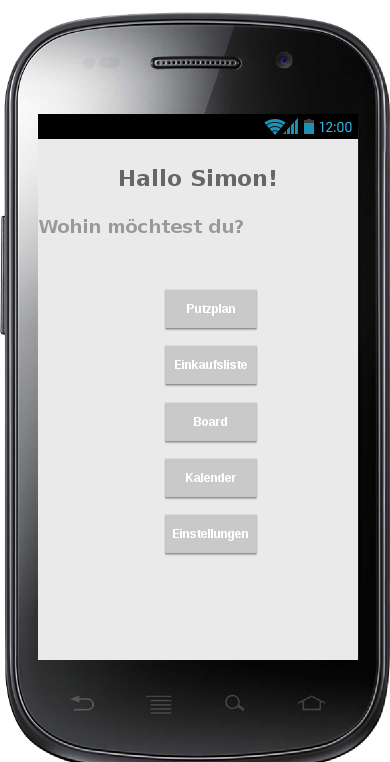
\includegraphics[width=0.7\textwidth]{anhang/mockups/overview.png}
  \caption{Erstes Bild}
  \label{fig:Bild1}
\end{figure}

\begin{figure}[htbp] 
  \centering
     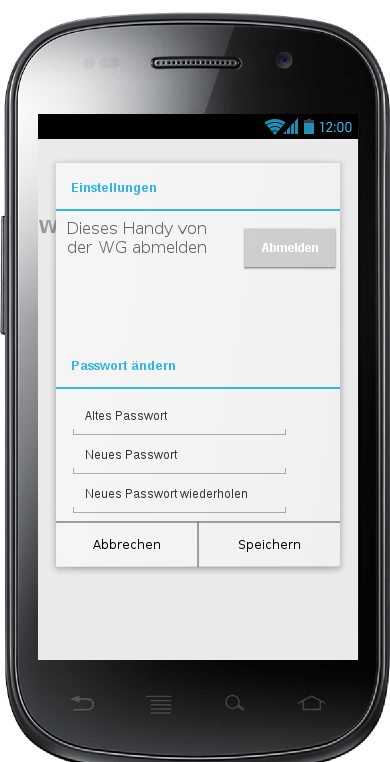
\includegraphics[width=0.7\textwidth]{anhang/mockups/overviewsettings.png}
  \caption{Erstes Bild}
  \label{fig:Bild1}
\end{figure}

\begin{figure}[htbp] 
  \centering
     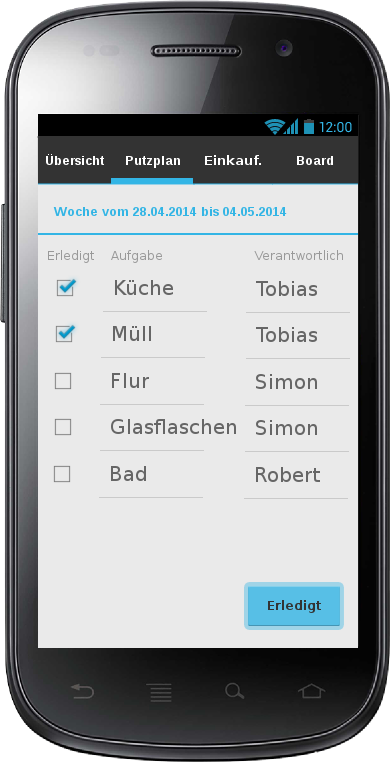
\includegraphics[width=0.7\textwidth]{anhang/mockups/putzplan.png}
  \caption{Erstes Bild}
  \label{fig:Bild1}
\end{figure}

\begin{figure}[htbp] 
  \centering
     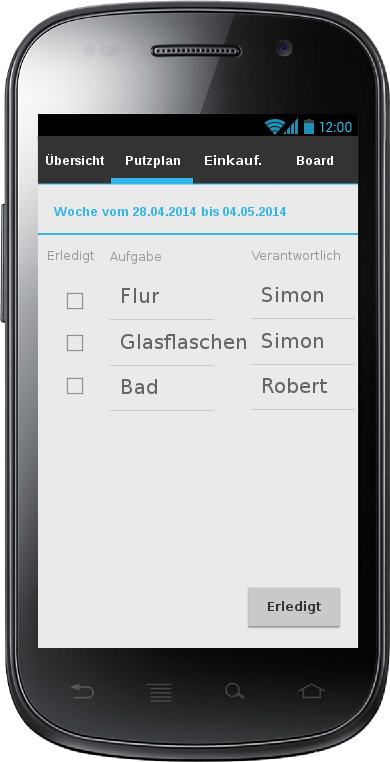
\includegraphics[width=0.7\textwidth]{anhang/mockups/putzplanerledigt.png}
  \caption{Erstes Bild}
  \label{fig:Bild1}
\end{figure}

\begin{figure}[htbp] 
  \centering
     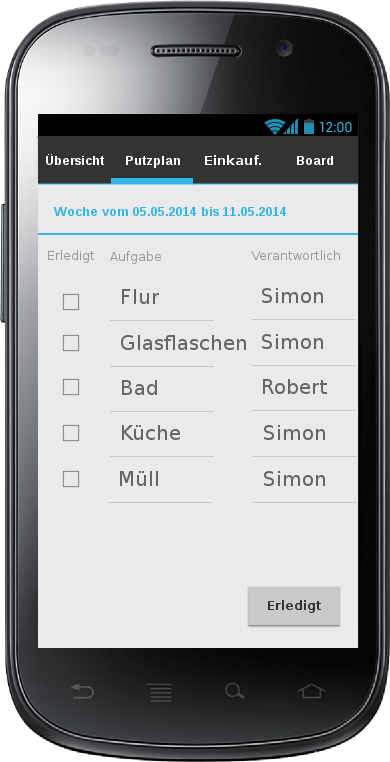
\includegraphics[width=0.7\textwidth]{anhang/mockups/putzplanneuewoche.png}
  \caption{Erstes Bild}
  \label{fig:Bild1}
\end{figure}

\begin{figure}[htbp] 
  \centering
     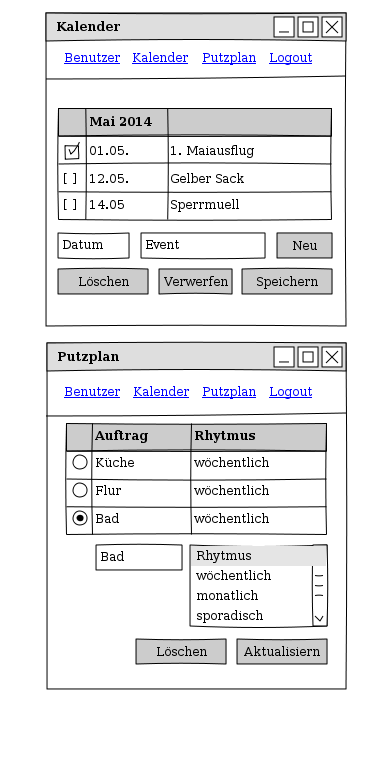
\includegraphics[width=0.7\textwidth]{anhang/mockups/webpage_1.png}
  \caption{Erstes Bild}
  \label{fig:Bild1}
\end{figure}

\begin{figure}[htbp] 
  \centering
     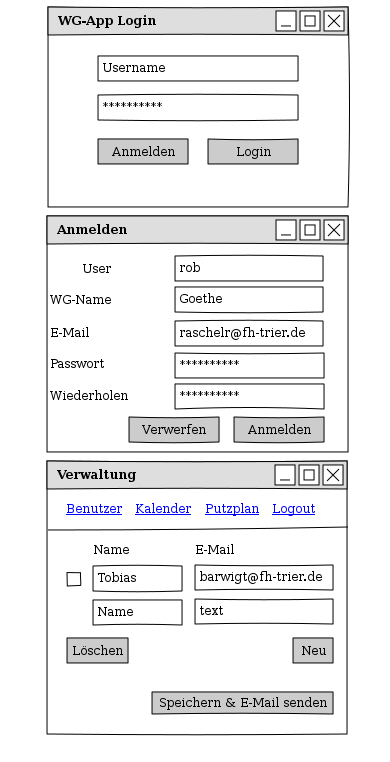
\includegraphics[width=0.7\textwidth]{anhang/mockups/webpage.png}
  \caption{Erstes Bild}
  \label{fig:Bild1}
\end{figure}

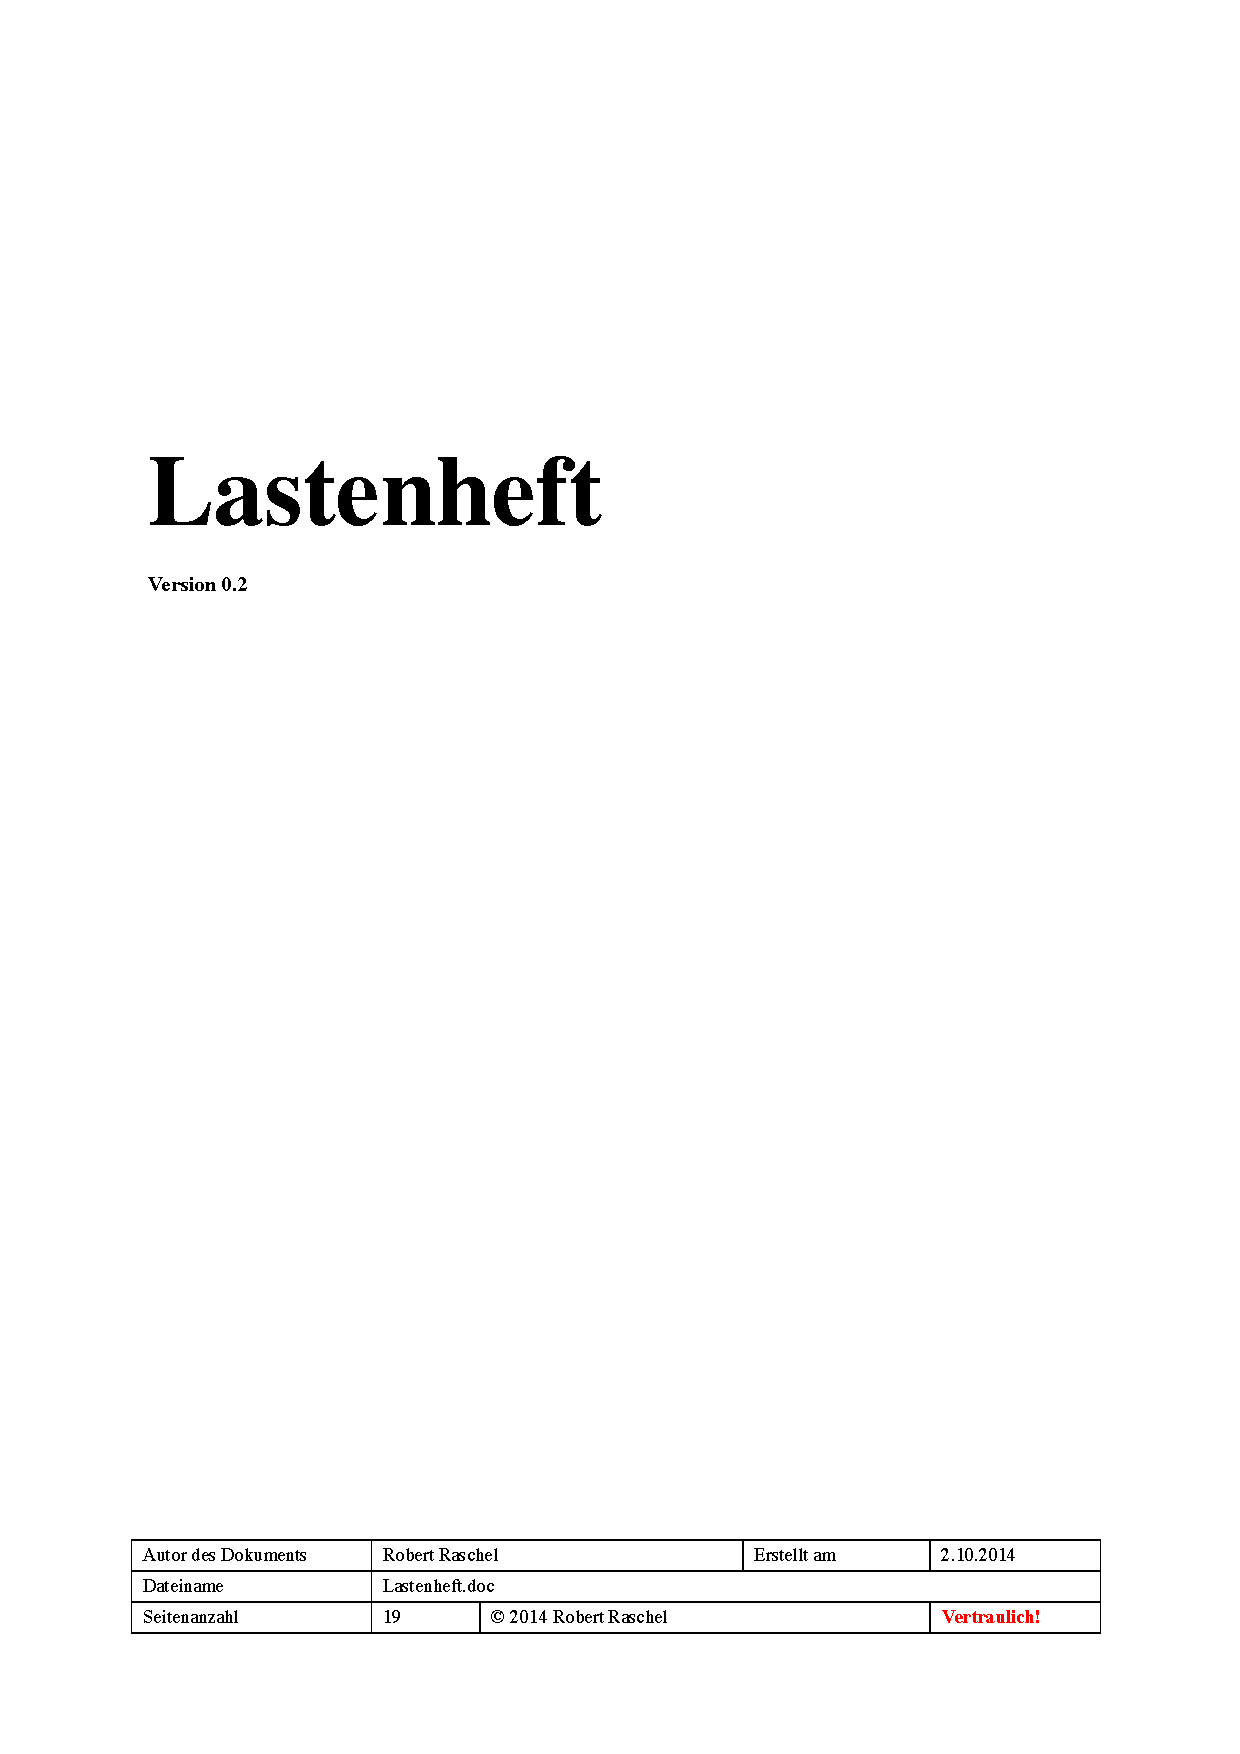
\includepdf[pages=-, addtotoc={1,section,1,Lastenheft,chap:int},  scale=0.85, pagecommand={}]{anhang/Lastenheft.pdf} 
%\includepdf[pages=2-, addtotoc={1,chapter,0,Lastenheft,chap:int},  scale=0.85, pagecommand={}]{anhang/Lastenheft.pdf} 

